%%=============================================================================
%% chapters/chapter5.tex — Digital-Twin-Based Validation (final-defense version)
%%=============================================================================
\chapter{Digital-Twin-Based Validation with Spatial-Operation Robots}
\label{ch:validation}
This chapter presents the third part of the framework: the architecture
through which the semantic database produced by Chapters~\ref{ch:mapping}
and~\ref{ch:semantic} is connected to a digital twin, a management console, and
a physical spatial-operation robot, so that the integrated framework can be
evaluated as a whole.\footnote{The content of this chapter is based on the author's RAAICON~2026 paper~\cite{raaicon2026} and on the application section of the TLS-SMF manuscript submitted to \emph{Electronics}~\cite{kim2026electronics}.} Section~\ref{sec:dt-arch} states the architecture and
its single-store principle. Section~\ref{sec:scan2sim} describes the automated
scan-to-simulation pipeline that turns the registered scan into a
physics-enabled NVIDIA Isaac Sim stage, Section~\ref{sec:twin-bridge} the live
bidirectional bridge and its frame calibration, Section~\ref{sec:semantic-twin}
the injection of the semantic layer into the twin, Section~\ref{sec:missions}
the semantic mission stack, and Section~\ref{sec:real-robot} the integration
with the physical robot.

\section{Validation Architecture and Single-Store Principle}
\label{sec:dt-arch}

The crux of the validation is to confirm that a single environmental
representation simultaneously satisfies different modes of consumption. The
knowledge graph of Chapter~\ref{ch:semantic} is the \emph{single semantic
store}: the management console (a browser interface that issues mission
commands, shows the live graph and robot state, and gives the owner one-click
refute/re-type/attribute edits), the semantic mission mediator, the Isaac Sim
twin, and---through the same mediator---the physical robot all read the same
revisioned file, so a correction propagates to every consumer from a single
write (Figure~\ref{fig:dt-arch}). Consistent with the laboratory's
RaaS-oriented control server~\cite{kwon2025}, the digital twin acts as the
supply layer from which a semantic task manager draws the environmental
knowledge required for cost-aware task allocation; where the task manager
decomposes natural-language commands and allocates them to heterogeneous
robots, the present framework supplies the underlying environmental knowledge
that such allocation depends upon. The validation of this chapter therefore
aims to demonstrate that the framework's output is not merely a visualizable
model but a representation that is consumable for actual robot mission
execution.

\begin{figure}[!htb]
  \centering
  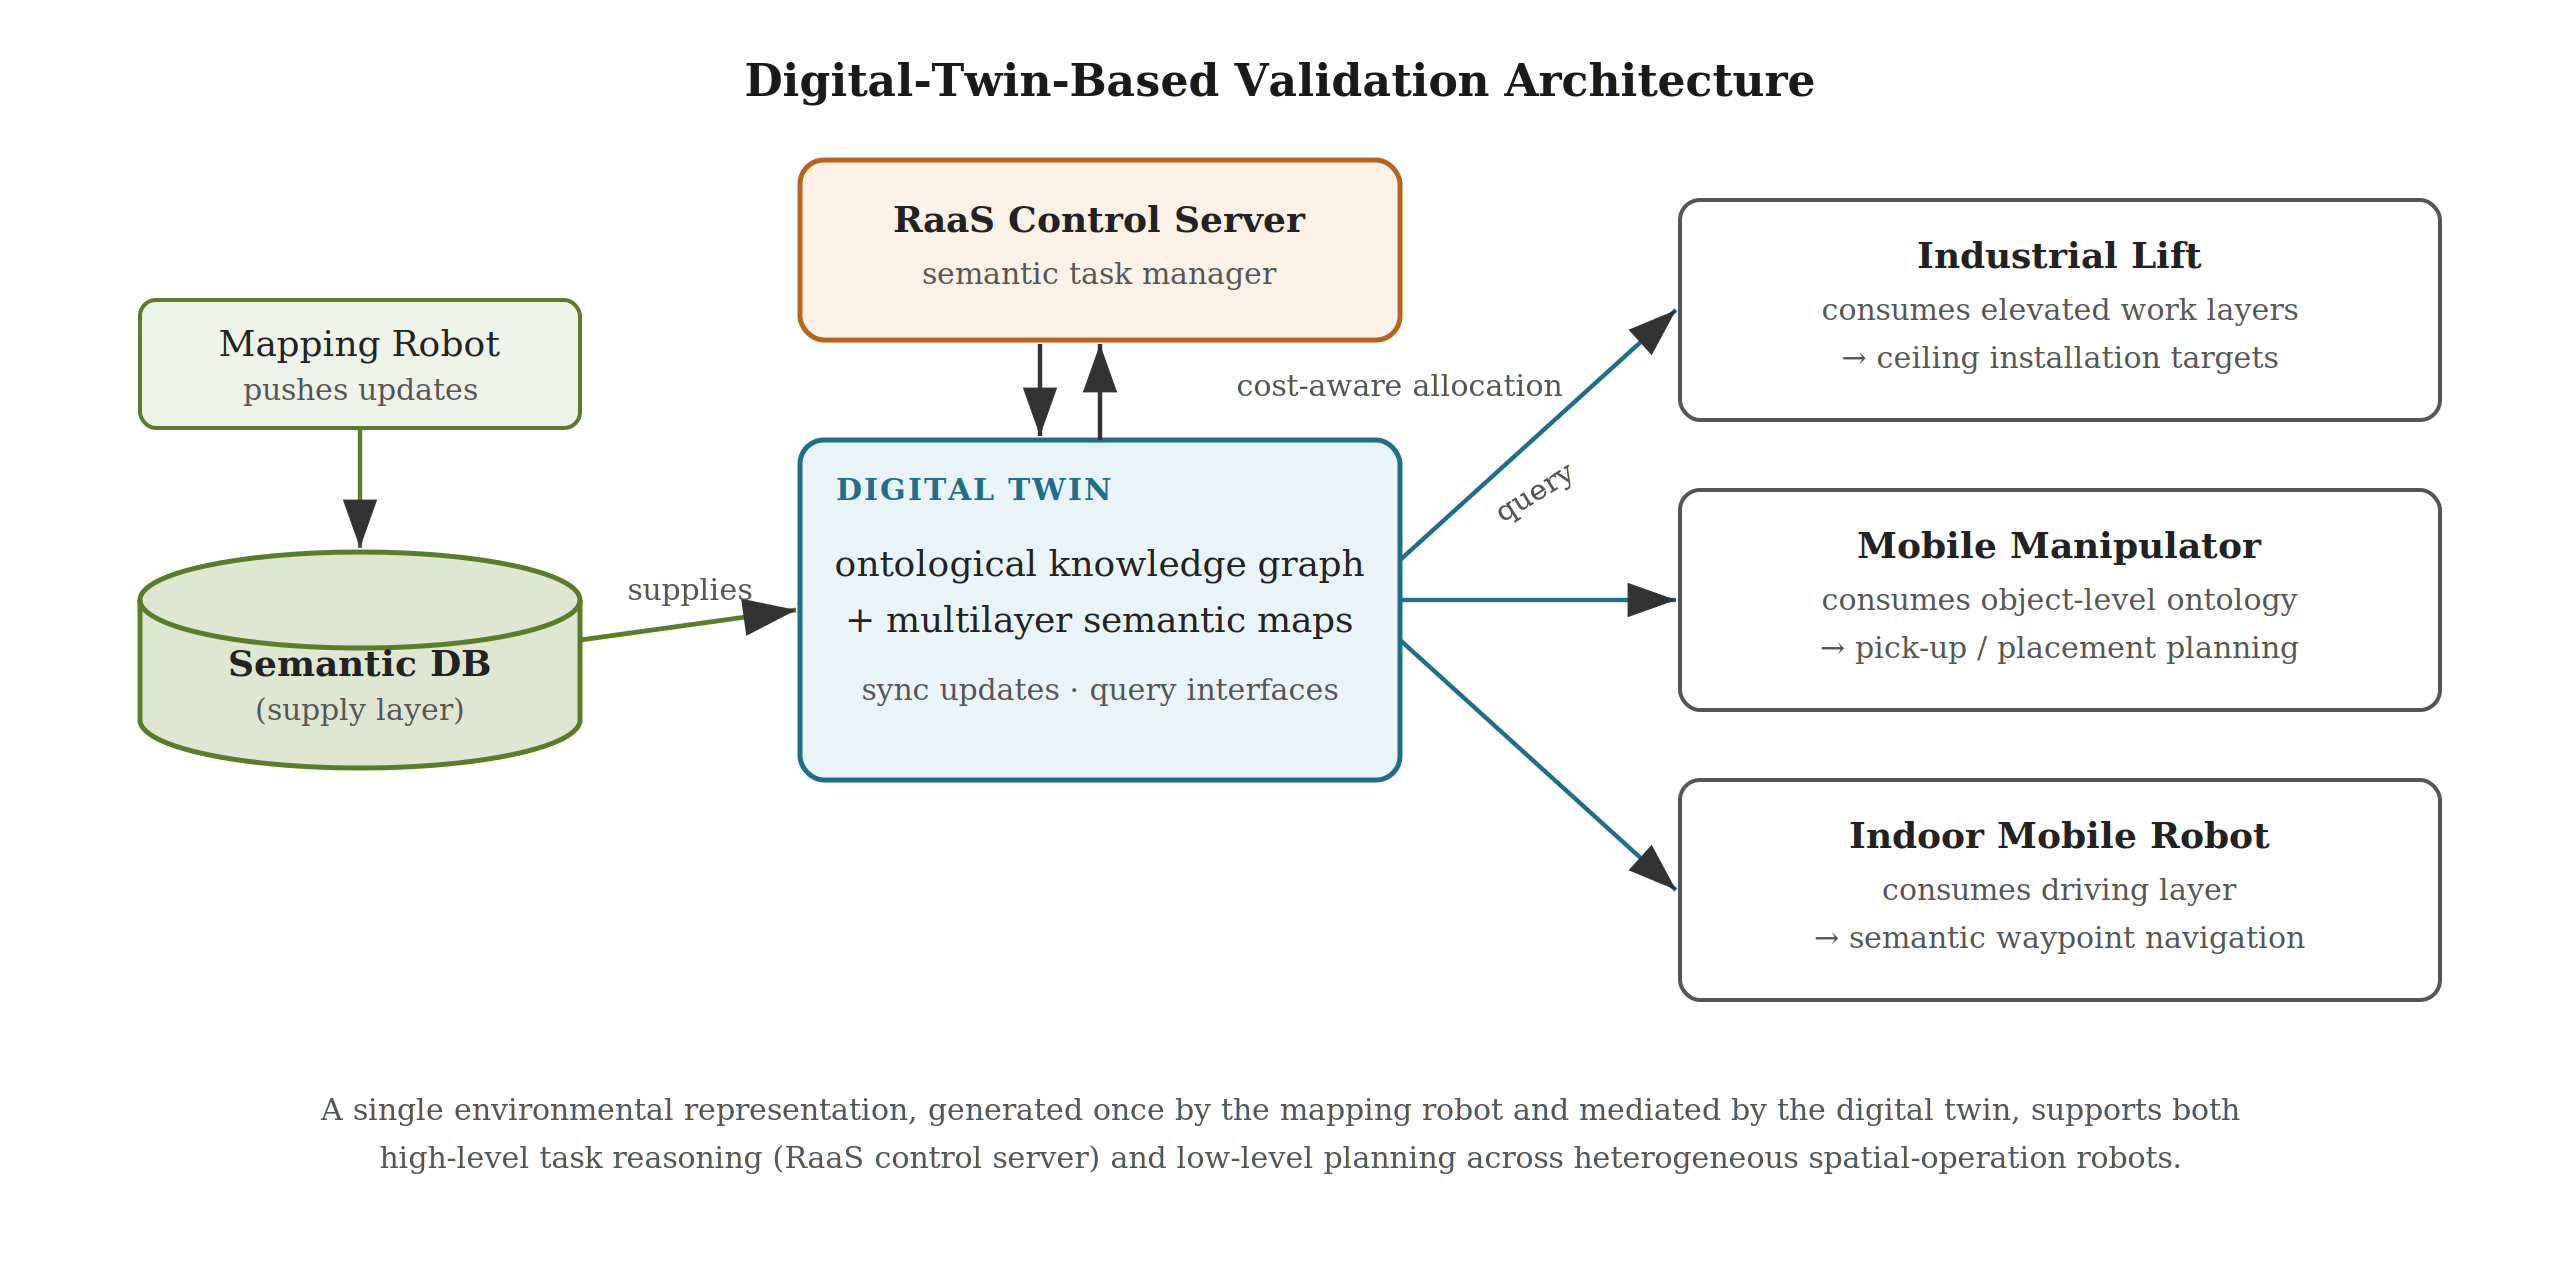
\includegraphics[width=0.95\textwidth]{figures/fig5_1.png}
  \caption{Digital-twin-based validation architecture. The semantic database
  supplies a digital twin connected to a RaaS-oriented control server;
  downstream robots consume the shared representation through query
  interfaces. In this dissertation the chain is validated with a swerve-drive
  mobile manipulator (AMMR), a single platform that spans the driving,
  manipulation, and overhead bands of the same store.}
  \label{fig:dt-arch}
\end{figure}

The validation platform is the AMMR, a swerve-drive autonomous mobile
manipulator robot deployed in the industrial test room in which all
experiments are conducted. A mobile manipulator is a natural single-platform
consumer of the multilayer representation of Section~\ref{sec:layers}: its
base navigates on the driving layer, its arm operates in the manipulation work
layer, and its end effector can be directed at targets in the overhead layer.
The experiments of Chapter~\ref{ch:experiments} exercise the driving band end
to end on hardware (console-issued semantic missions) and the manipulation and
overhead bands at the representation level (verified object poses and
footprints at reach height, and ceiling-mounted structure recognized from the
same scan), which is the contract a manipulation or installation planner
consumes.

\section{Scan-to-Simulation Pipeline}
\label{sec:scan2sim}

Constructing a simulation environment that faithfully reproduces a real
indoor workspace is a major bottleneck when deploying digital twins: scenes are
typically modeled by hand, which is slow, subjective, and quickly outdated. A
raw point cloud is not a simulation environment either: it has no collision
representation, no gravity-aligned reference frame, and no interface to a
robot simulator. The pipeline of Figure~\ref{fig:raa-pipeline} converts the
merged E57 export automatically into a physics-ready Isaac Sim USD stage. It
deliberately keeps two decoupled layers---a coarse collision layer derived
from the occupancy grid and a dense point layer for appearance---which keeps
conversion fast, robust to scan noise, and directly navigable by a mobile base,
rather than reconstructing a watertight mesh.

\begin{figure}[!htb]
\centering
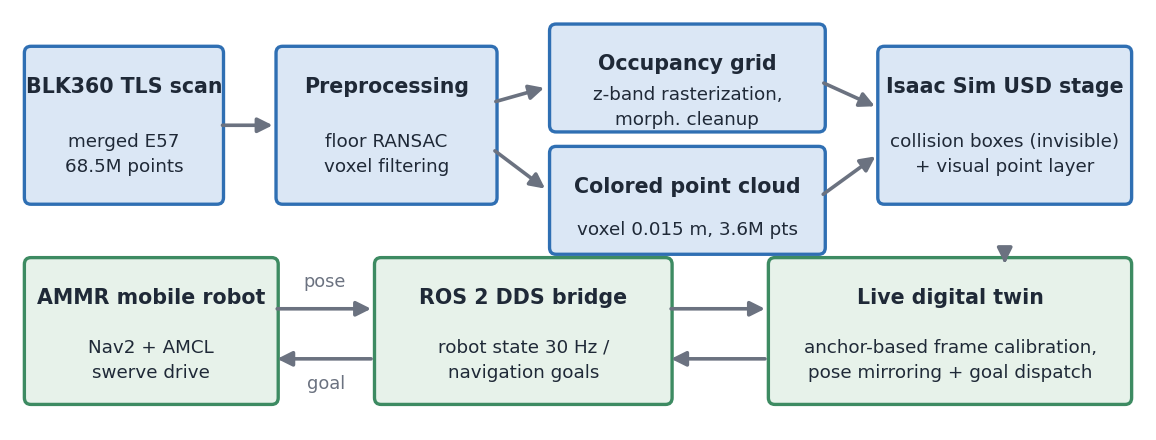
\includegraphics[width=0.9\linewidth]{figures/raa_fig_pipeline.png}
\caption{Scan-to-simulation system overview. Offline (top): the merged BLK360
E57 export is converted into an occupancy grid, a collidable wall layer, and a
dense colored point layer composing the Isaac Sim stage. Online (bottom): a
ROS~2 DDS bridge mirrors the robot pose at 30~Hz and returns navigation goals
selected in the simulator.}
\label{fig:raa-pipeline}
\end{figure}

\subsection{Preprocessing and Floor-Plane Estimation}
\label{subsec:s2s-preproc}

The pipeline first estimates the dominant floor plane with RANSAC on a
voxel-thinned subset of the merged cloud, yielding the gravity-aligned
reference frame and the floor height $z_0$; all subsequent layers are expressed
relative to this frame, so no manual leveling or origin selection is required.
In the test room, the registered stations were exported as a single E57 file
of 68.5~M points (1.3~GB); scan placement followed the visibility-coverage plan
of Chapter~\ref{ch:mapping}.

\subsection{Occupancy Grid and Collision Layer}
\label{subsec:s2s-occ}

Points within the height band $[z_0{+}0.10,\ z_0{+}1.80]$~m---the band relevant
for a mobile base---are rasterized into a 2D occupancy grid at 0.05~m
resolution. Morphological cleanup removes speckle from reflections and small
blobs below 0.02~m$^2$. The occupied cells are then greedily merged into
axis-aligned boxes and emitted as USD cubes of 2.5~m height with physics
collision enabled. Crucially, the collision boxes are marked \emph{invisible}:
they provide physics without occluding the visual point layer. The same
occupancy grid is exported in the ROS map format so that the simulated and real
navigation stacks can share one map; it is the driving layer of
Section~\ref{sec:layers}.

\subsection{Visual Point-Cloud Layer}
\label{subsec:s2s-visual}

For appearance, the full-resolution colored cloud is voxel-downsampled to
0.015~m (3.6~M points, ceiling included) and embedded as USD point primitives
with per-point color and a rendered point width of 0.013~m, chosen at
approximately 0.85 times the voxel size so that points visually fuse into
surfaces at navigation-relevant viewing distances. The two-layer design keeps
the stage lightweight: collision queries run against about 1{,}430 boxes rather
than millions of points, while the operator sees the photographic appearance of
the real room.

\subsection{Robot Model and Mobile-Base Control}
\label{subsec:s2s-robot}

The AMMR is a swerve-drive mobile manipulator with two independently steered
wheel modules mounted diagonally at $\mathbf{p}_{1,2}=(\pm0.364,\ \mp0.137)$~m
and four passive casters; its URDF (12 links, 11 joints) was authored from the
manufacturer's 2D drawings. For simulation-only operation the base is
velocity-controlled through the standard inverse kinematics: for a commanded
body twist $(v_x, v_y, \omega)$ each module $i$ tracks
\begin{equation}
\mathbf{v}_i = \begin{bmatrix} v_x - \omega\, p_{i,y} \\
v_y + \omega\, p_{i,x} \end{bmatrix},\quad
\delta_i = \operatorname{atan2}(v_{i,y}, v_{i,x}),\quad
\dot\varphi_i = \frac{\lVert \mathbf{v}_i \rVert}{r},
\label{eq:swerve}
\end{equation}
with wheel radius $r=0.075$~m. Steering angles are wrapped to
$[-90^\circ, 90^\circ]$ with wheel-speed reversal; a hysteresis of 0.12~rad on
the reversal decision and a cosine speed gate suppress the flip-flopping that
otherwise occurs when a module operates exactly at the wrap boundary, for
example during pure rotation. The TOSM robot layer (footprint, drive type,
sensor mounts, velocity limits) is instantiated from the same URDF and
navigation configuration and ingested alongside objects and places, completing
the three-element TOSM model; the same layer drives the Gazebo proxy of
Section~\ref{sec:missions}.

\section{Live Twin Bridge and Frame Calibration}
\label{sec:twin-bridge}

During live operation the simulated robot is switched to kinematic mode and
mirrors the real pose. The robot publishes its localized pose (AMCL
localization~\cite{dellaert1999} on its own navigation map) as a 30~Hz
odometry stream; the simulator subscribes over a DDS bridge (Cyclone
DDS~\cite{cyclonedds}, a dedicated ROS~2 domain, unicast peer configuration
over Wi-Fi) and applies the pose each physics step. In the reverse direction,
dragging a goal marker in the simulator publishes a goal pose that an on-robot
relay forwards to the robot's Nav2 stack~\cite{macenski2020marathon}, closing
the loop: the physical robot navigates to targets picked in the twin.

The robot's SLAM map frame and the scan frame differ by an unknown planar rigid
transform. It is calibrated with a single anchor: the robot is parked at a
physically identifiable spot whose scan-frame pose $(\mathbf{a}, \theta_a)$ is
known---in the test room the robot itself was captured in the scan, so its
scanned footprint provides the anchor; a taped start spot of known scan
coordinates serves the same purpose in later sessions. On receipt of the first
live pose $(\mathbf{r}, \theta_r)$ the offset follows in closed form,
\begin{equation}
\theta_{\mathrm{off}} = \theta_a - \theta_r, \qquad
\mathbf{t}_{\mathrm{off}} = \mathbf{a} - R(\theta_{\mathrm{off}})\,\mathbf{r},
\label{eq:anchor}
\end{equation}
and is reused for all subsequent poses and goals. The one-shot calibration
inherits the localization error of the single pose sample it is computed from:
any AMCL error at anchor time becomes a permanent bias of the session, and
across on-site sessions the recovered offsets differed by up to 0.60~m and
$9.1^\circ$, reflecting run-to-run differences in AMCL initialization rather
than scene error. The operating procedure therefore verifies the overlay
visually after anchoring (a short teleoperated advance must move the twin in
the same direction as the robot) and re-anchors if the twin is misaligned.
Averaging over multiple anchor poses, or refining the offset by matching the
live 2D-lidar scan against the TLS cloud, would remove the single-sample
dependence.

\section{Semantic Twin Injection}
\label{sec:semantic-twin}

Because every node of the knowledge graph carries an explicit model in the
scan frame, the graph can be injected directly into the simulation stage. The
digital twin of Section~\ref{sec:scan2sim} is extended with the semantic
layer: the stage is re-derived from the graph whenever the graph changes, each
verified object spawning a labeled proxy (extent box or segmented cloud) with
its verification status, provenance, height level, and label stability exposed
in a scene inspector, while unverified objects spawn as neutral gray
placeholders---the gate is visible in the twin. A file watcher converts the
current graph revision to a USD layer and the running stage reloads it, so an
owner edit in the console propagates to the robot's next goal, the console,
and the twin from one write. The discipline is self-auditing: deriving the
stage from the graph immediately visualized eighteen stale earlier-epoch nodes
as orphan boxes that per-view export paths had silently hidden, prompting the
cleanup revision reported in Section~\ref{sec:exp-update}.

\section{Semantic Mission Stack}
\label{sec:missions}

The loop from scan-derived knowledge to autonomous behavior is closed by a
mission stack with three components. A \emph{semantic mediator} resolves
high-level mission commands---\texttt{goto\_place}, \texttt{goto\_object},
\texttt{patrol}, \texttt{return\_home}---against the knowledge graph: places
resolve to free-space points at region centroids, objects to approach poses
computed from the target's footprint and the robot's circumscribed radius (the
kinematics-aware resolution style of TOSMNav~\cite{joo2022fsom}), with the
verification gate deciding eligibility; a command that resolves to an
unverified or refuted node is refused in under one second with no motion. The
mediator covers command resolution only; full hierarchical task planning over
the same TOSM knowledge is the natural next consumer of the graph and is out
of scope. A hybrid deliberative/reactive \emph{behavior
tree}~\cite{colledanchise2018bt,iovino2022btsurvey} (Figure~\ref{fig:bttree})
executes the resolved goals through Nav2, with a reactive layer that preempts
the mission on low battery, an operator stop, or an interrupt and returns the
robot to its home pose. The \emph{management console} issues commands, shows
the live robot pose and status log, and edits the graph live; the mediator
hot-reloads owner edits, so refuting a phantom in the console changes robot
behavior on the next command without a restart.

\begin{figure}[!htb]
\centering
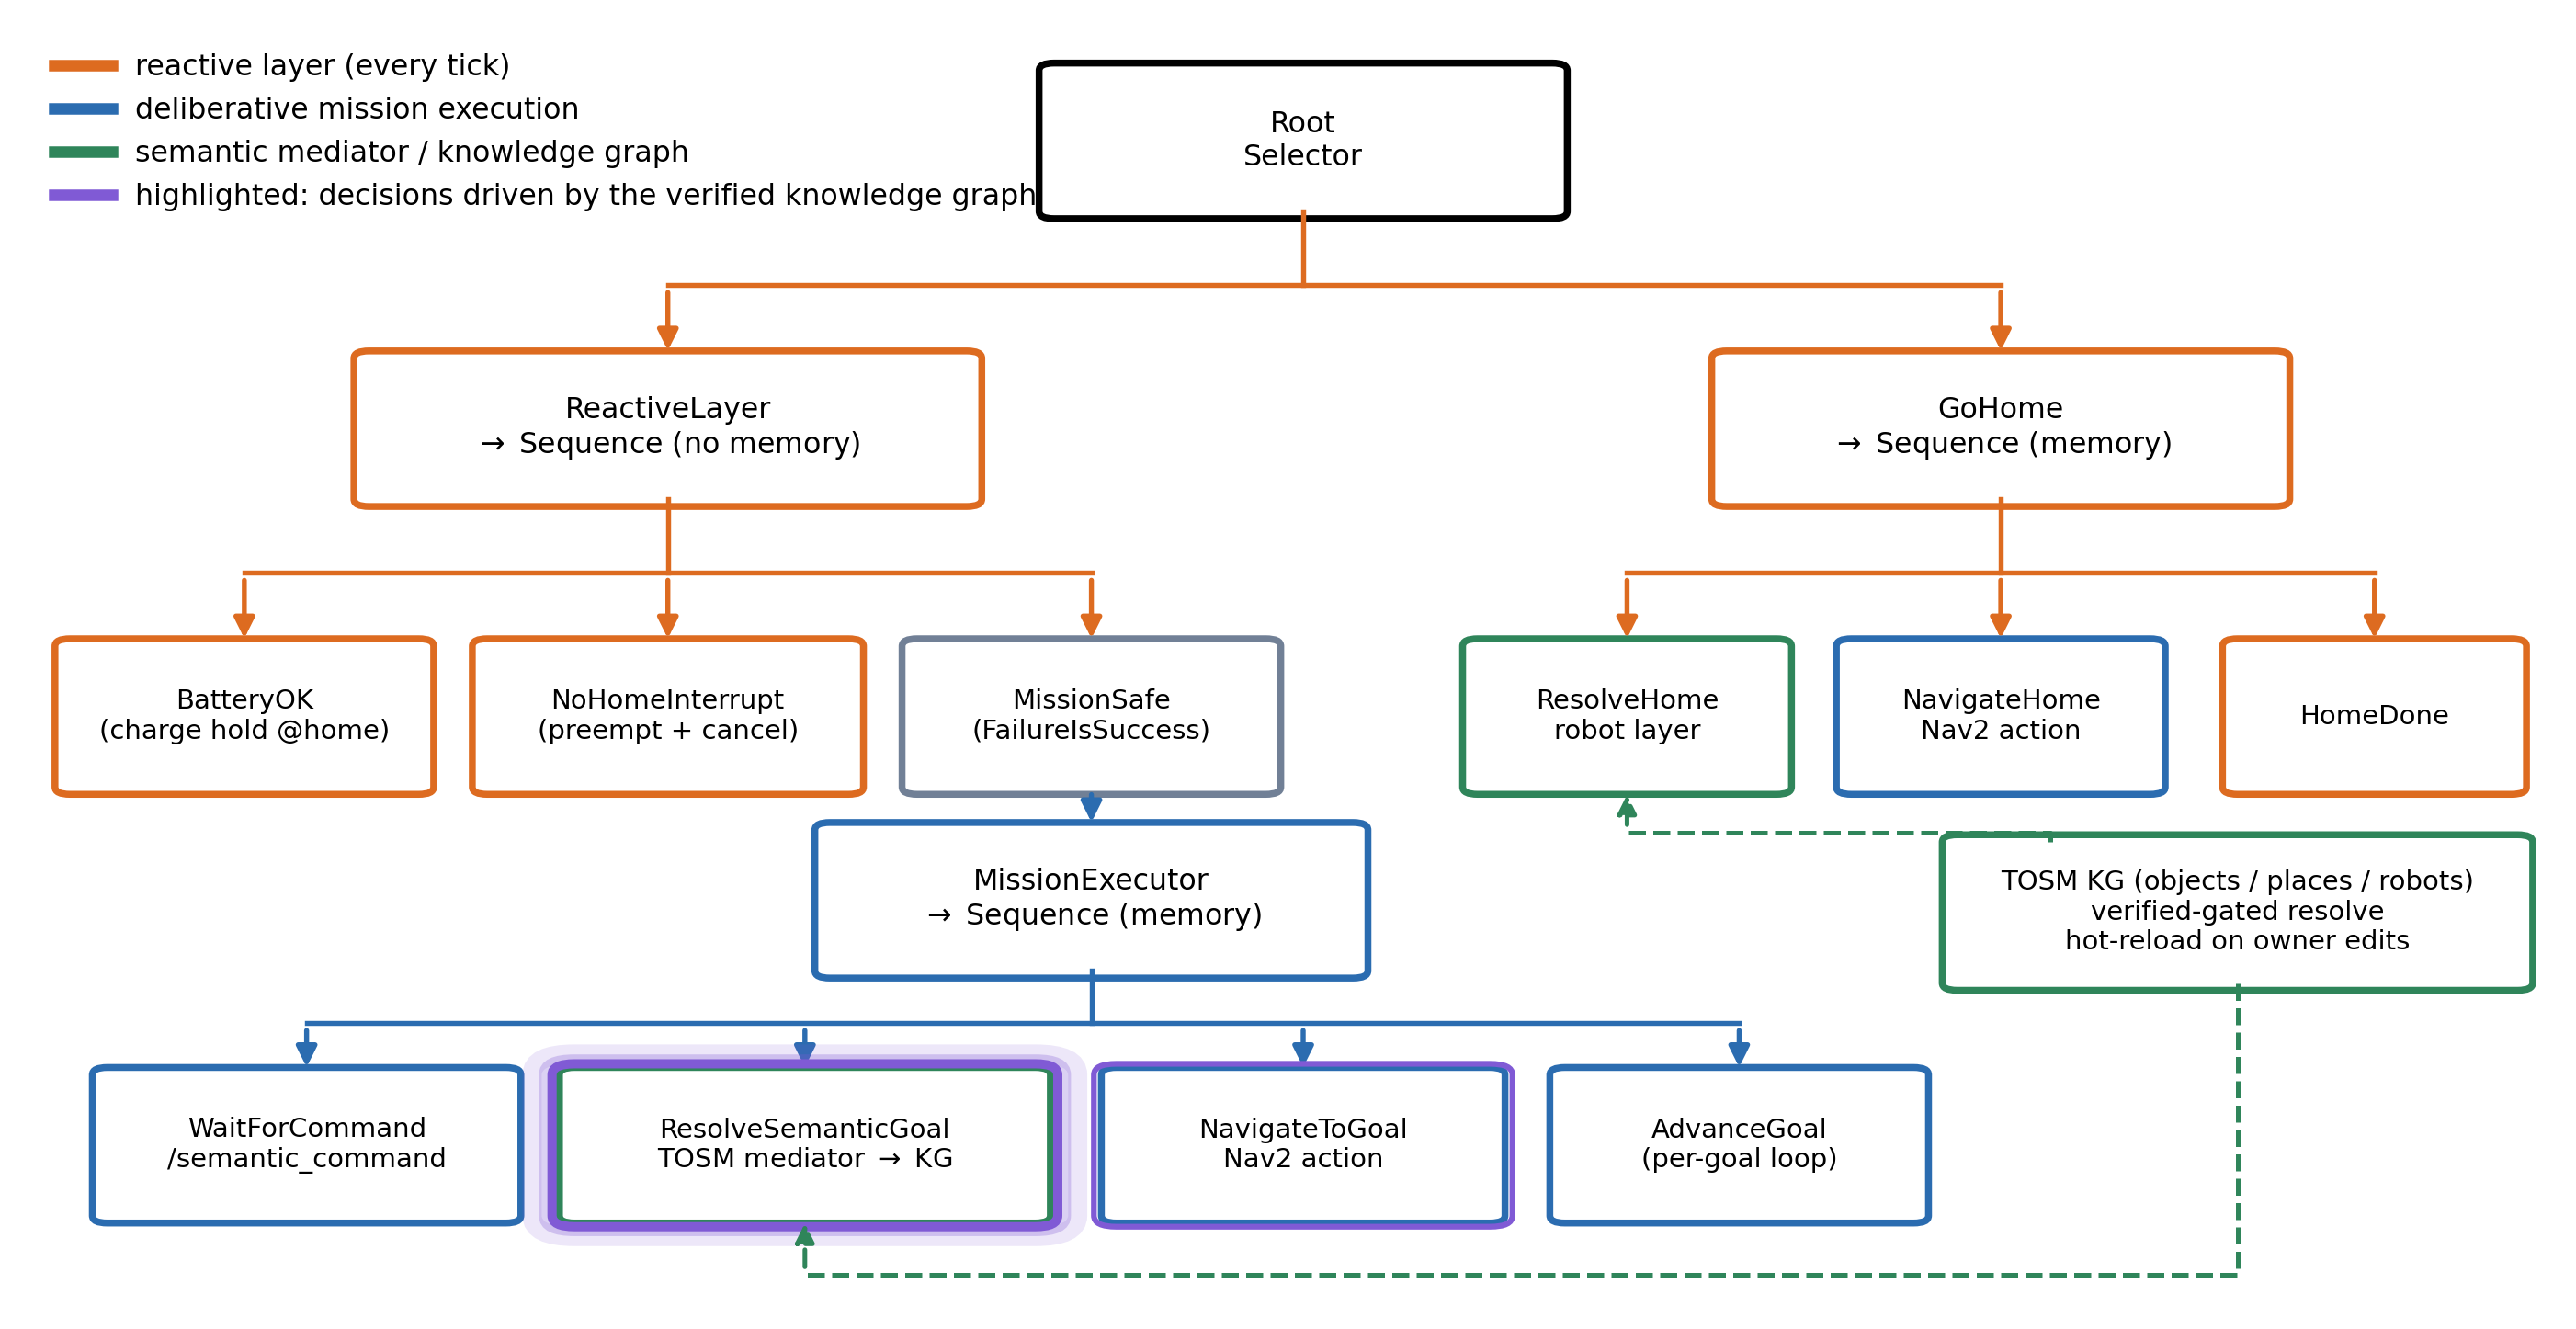
\includegraphics[width=0.9\linewidth]{figures/ele_fig16_bt_tree.png}
\caption{Hybrid deliberative/reactive mission behavior tree. The reactive
layer re-evaluates battery, stop, and interrupt conditions every tick and can
preempt navigation (canceling the active Nav2 goal); the deliberative branch
resolves semantic commands through the TOSM mediator, which hot-reloads the
knowledge graph when the management console edits it. Highlighted nodes are
the decisions the verified knowledge graph drives: the semantic-resolve node,
where a gated graph refuses phantom or unverified goals, and the navigation
node that consumes the resolved pose.}
\label{fig:bttree}
\end{figure}

In simulation, the stack runs in a Gazebo~\cite{koenig2004gazebo} world
generated from the same exploration occupancy grid that anchors the place
layer, so world, navigation map, and knowledge graph share one frame. The
simulated vehicle is a digital proxy of the target platform: the AMMR's
footprint ($1.25\times0.8$~m), lidar mount, and velocity limits from the TOSM
robot layer are instantiated in the world, and the mediator derives approach
poses and clearance checks (circumscribed radius 0.74~m) from the same
layer---the knowledge that \emph{describes} the robot is the knowledge that
\emph{drives} it.

\section{Real-Robot Integration}
\label{sec:real-robot}

To close the loop on hardware, the mission stack of Section~\ref{sec:missions}
is run unchanged against the physical AMMR, with the knowledge graph as the
semantic store. The platform runs its own localization and Nav2 stack on an
independently built occupancy map; a thin bridge node replaces the simulator.
It converts the robot's localization pose into the scan frame through the
single SE(2) offset of Equation~\ref{eq:anchor}, calibrated once by parking the
robot on a taped start spot of known scan coordinates, and republishes it as the
pose the mediator and the twin consume; in the reverse direction it exposes
the navigation action interface the behavior tree expects, forwards the
mediator's resolved goals (scan frame) to the robot's on-board navigation in
the robot's map frame, monitors arrival within a tolerance radius with a short
settling time, and implements the console's stop command by canceling the
active mission and holding the current pose. Nothing above the bridge changes:
commands are issued from the management console, the mediator resolves and
gates them against the graph, the behavior tree executes them, and the Isaac
Sim twin mirrors the robot from the same store. Because the robot reports its
heading in its own map convention, the bridge also applies a fixed heading
offset determined during the anchoring check. The measured outcomes of this
integration---conversion time, simulation throughput, geometric fidelity,
simulator-issued goal trials, and console-issued semantic missions on the
physical robot---are reported in Sections~\ref{sec:exp-twin}
and~\ref{sec:exp-missions}.
